\documentclass{article}

\usepackage{graphicx}
\usepackage{tikz}
\usepackage{tikzsymbols}
\usetikzlibrary{calc,patterns,shapes.geometric}
\pagestyle{empty}
\usepackage[margin=0pt]{geometry}
\geometry{papersize={14in,12in}}

\def\centerarc[#1](#2)(#3:#4:#5){\draw[#1] ($(#2)+({#5*cos(#3)},{#5*sin(#3)})$) arc (#3:#4:#5);}

\begin{document}
	\begin{figure}
		\centering
		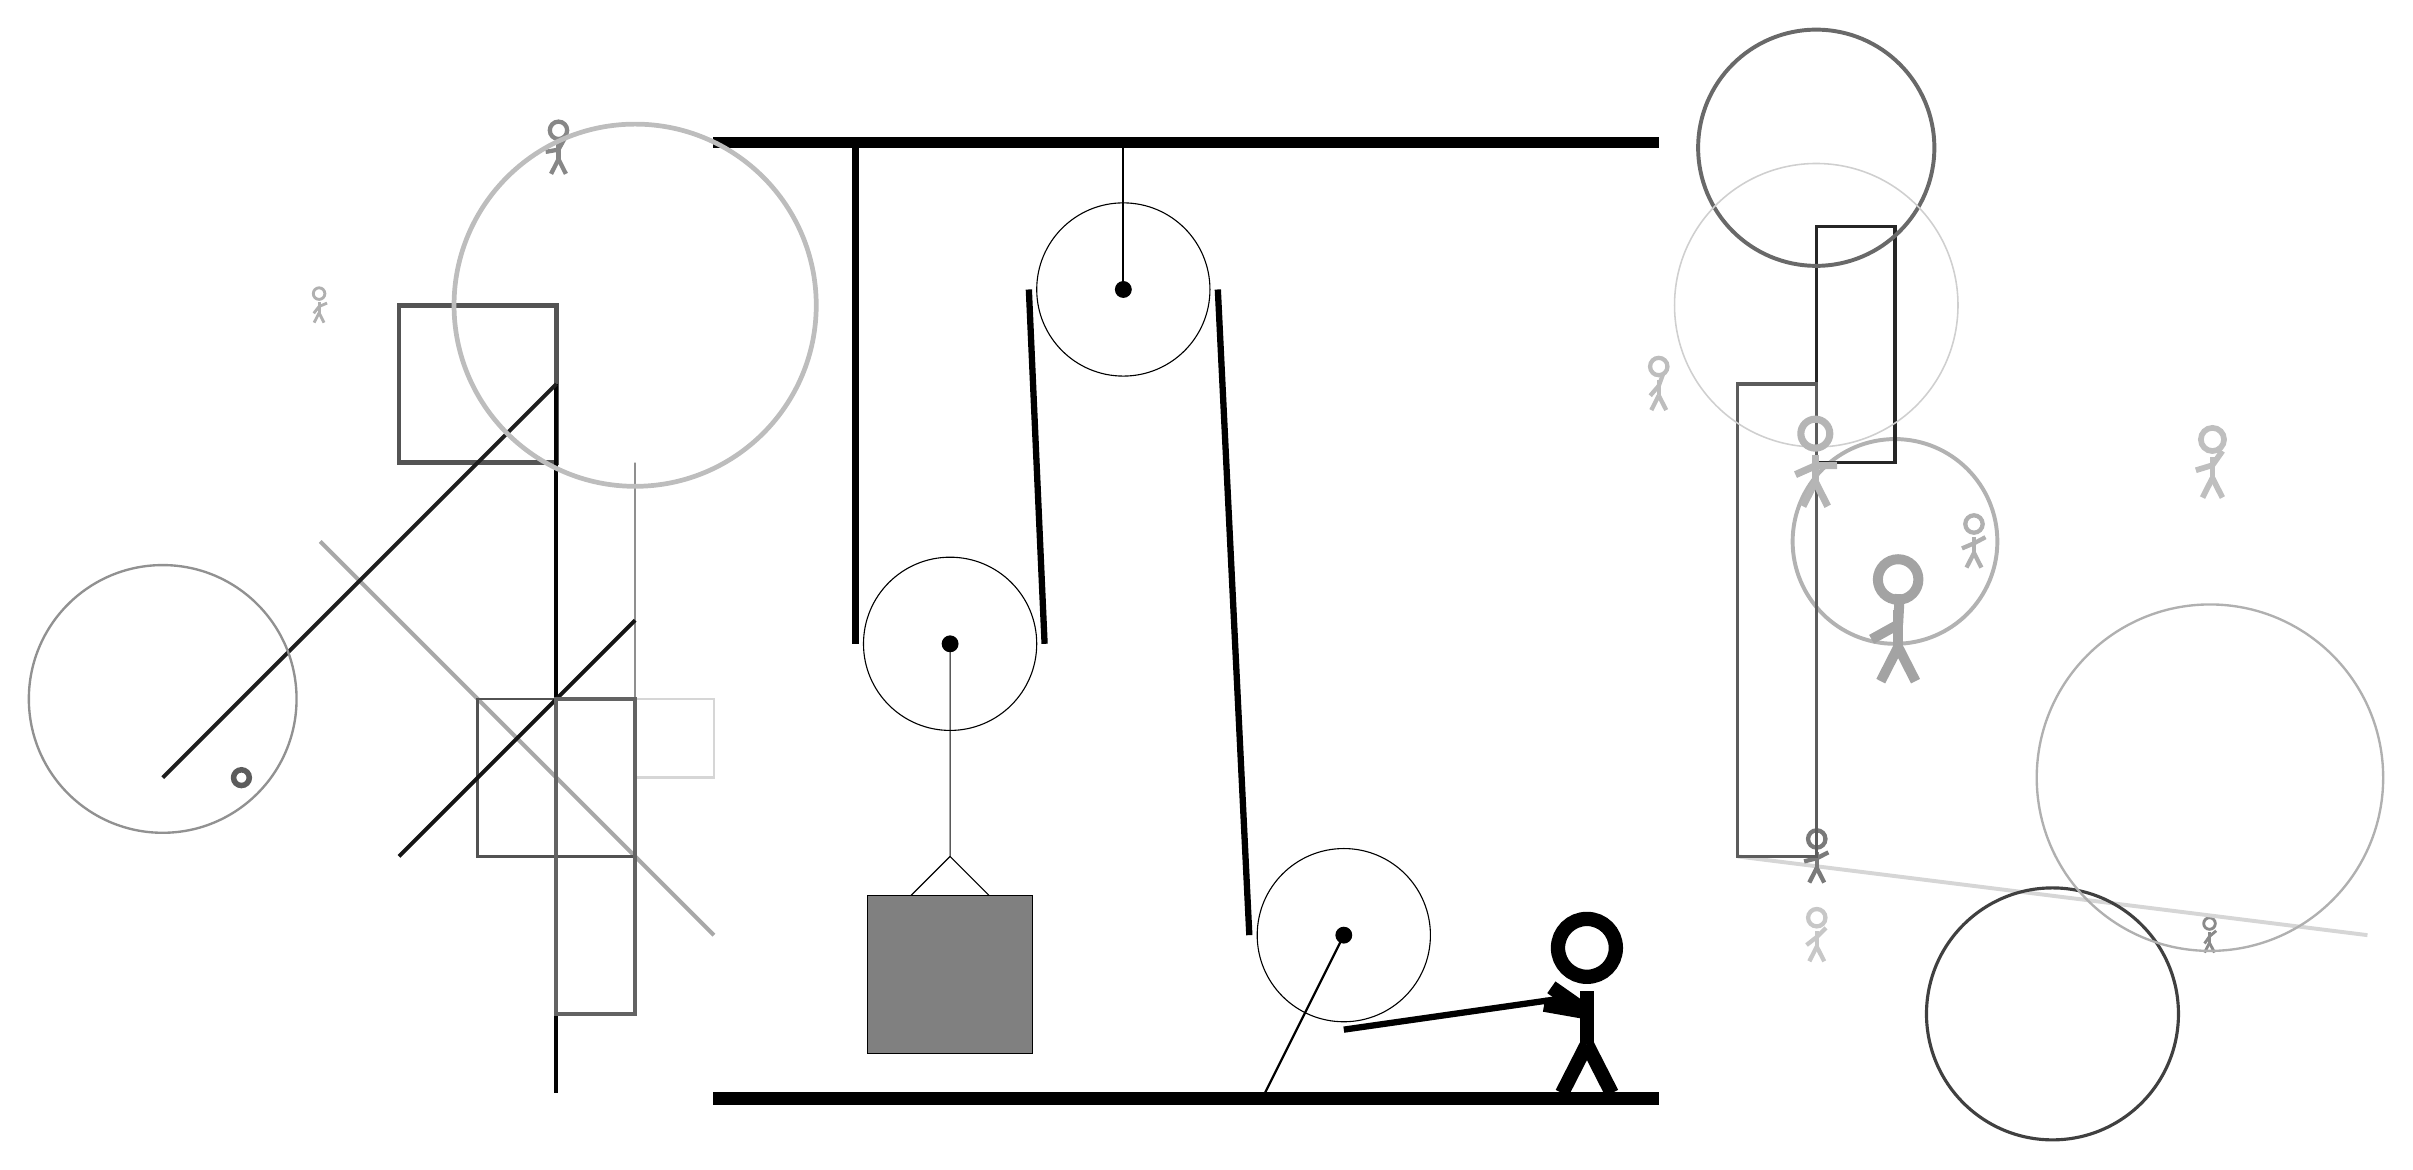
\begin{tikzpicture}
			%%%%% START %%%%%
			
			\draw[fill=black] (-2, 9) rectangle (10, 9.125);
			
			\draw (3.2, 7.2) circle (1.1);
			\draw[fill=black] (3.2, 7.2) circle (0.1);
			\draw[thick] (3.2, 7.2) -- (3.2, 9);
			
			\draw [line width=0.7mm, color=black!64](-8, 1) circle (0.1);
			
			\draw[line width=0.2mm, color=black!44] (-3, -1) rectangle (-3, 5);
			\node[line width=0.2mm, color=black!46] at (17, -1) {\Strichmaxerl[2][55][40]};
			\node[line width=0.7mm, color=black!31] at (14, 4) {\Strichmaxerl[3][23][28]};
			\draw[line width=0.5mm, color=black!16](11, 0) -- (19, -1);
			
			\draw [line width=0.5mm, color=black!30](13, 4) circle (1.3);
			\draw[line width=0.5mm, color=black!34](-7, 4) -- (-2, -1);
			
			\draw[line width=0.6mm, color=black!67] (-4, 7) rectangle (-6, 5);
			\node[line width=0.2mm, color=black!31] at (-7, 7) {\Strichmaxerl[2][52][23]};
			\draw[line width=0.3mm, color=black!16] (-2, 1) rectangle (-3, 2);
			\draw[line width=0.4mm, color=black!85] (12, 5) rectangle (13, 8);
			
			\node[line width=0.3mm, color=black!47] at (-4, 9) {\Strichmaxerl[3][10][61]};
			\draw[line width=0.5mm, color=black!99](-4, 6) -- (-4, -3);
			\draw[line width=0.3mm, color=black!68] (-3, 2) rectangle (-5, 0);
			\draw[line width=0.5mm, color=black!92](-6, 0) -- (-3, 3);
			\draw [line width=0.5mm, color=black!59](12, 9) circle (1.5);
			
			\node[line width=0.7mm, color=black!52] at (12, 0) {\Strichmaxerl[3][14][27]};
			
			\draw[line width=0.5mm, color=black!61] (-3, 2) rectangle (-4, -2);
			\node[line width=0.7mm, color=black!25] at (17, 5) {\Strichmaxerl[4][17][55]};
			
			\draw[line width=0.5mm, color=black!88](-4, 6) -- (-9, 1);
			\draw[line width=0.4mm, color=black!64] (11, 0) rectangle (12, 6);
			
			\draw [line width=0.3mm, color=black!43](-9, 2) circle (1.7);
			\node[line width=0.3mm, color=black!36] at (13, 3) {\Strichmaxerl[7][29][87]};
			\node[line width=0.3mm, color=black!22] at (12, -1) {\Strichmaxerl[3][38][45]};
			\draw [line width=0.4mm, color=black!75](15, -2) circle (1.6);
			
			\draw [line width=0.2mm, color=black!19](12, 7) circle (1.8);
			\node[line width=0.3mm, color=black!29] at (12, 5) {\Strichmaxerl[5][24][1]};
			\draw [line width=0.6mm, color=black!26](-3, 7) circle (2.3);
			\draw [line width=0.3mm, color=black!31](17, 1) circle (2.2);
			\node[line width=0.2mm, color=black!26] at (10, 6) {\Strichmaxerl[3][49][70]};
			
			\draw (6, -1) circle (1.1);
			\draw[fill=black] (6, -1) circle (0.1);
			\draw[thick] (6, -1) -- (5, -3);
			
			\draw (1, 2.7) circle (1.1);
			\draw[fill=black] (1, 2.7) circle (0.1);
			
			\draw (1, 2.7) -- (1, 0) -- (0.5, -0.5);
			\draw (1, 0) -- (1.5, -0.5);
			\draw[fill=black!50] (-0.05, -0.5) rectangle (2.05, -2.5);
			
			\draw[line width=0.8mm] (-0.2, 9) -- (-0.2, 2.7);
			\centerarc[line width=0.8mm](1, 2.7)(180:360:1.2000000000000002);
			\draw[line width=0.8mm](2.2, 2.7) -- (2.0, 7.2);
			\centerarc[line width=0.8mm](3.2, 7.2)(0:180:1.2000000000000002);
			\draw[line width=0.8mm](4.4, 7.2) -- (4.8, -1);
			\centerarc[line width=0.8mm](6, -1)(180:270:1.2000000000000002);
			\draw[line width=0.8mm](6, -2.2) -- (8.8, -1.8);
			
			\node at (9, -1.9) {\Strichmaxerl[10][-35][170]};
			
			\draw[fill=black] (-2, -3) rectangle (10, -3.15);
			
			%%%%% END %%%%%
		\end{tikzpicture}
	\end{figure}	
\end{document}